\documentclass[12pt]{article}

%opening
\title{Tesina Segnali e Sistemi 2022}
\author{Lorenzo Franceschetti Mat. 2000263}
\date{}
\usepackage[margin=0.5in]{geometry}
\usepackage{graphicx}
%\graphicspath{ { ./images} }
\begin{document}

\maketitle

Sia dato il segnale $x_{t}(t)$, ottenuto dalla modulazione in ampiezza del segnale $x(t)$ alla frequenza $F_{m}$ tramite la seguente operazione: 
\begin{equation}
	x_{t}(t) = x(t) cos(2\pi F_{m}t)
\end{equation} 
Allora si può ottenere il segnale originale attraverso la seguente procedura:
\begin{itemize}
	\item Moltiplicare il segnale modulato per $2cos(2\pi F_{m}t)$
	\item Filtrare il segnale ottenuto tramite un filtro con risposta in frequenza data da
	\begin{equation}
		H_{lp}(f) = rect \biggl(\frac{f}{2B}\biggr)
	\end{equation}
	dove $B$ è la banda monolatera del segnale $x(t)$
\end{itemize}

La trasformata di Fourier $X_{t}(f)$ del segnale $x_{t}(t)$ risulta essere:\par
\begin{figure}[h!]
	\centering
	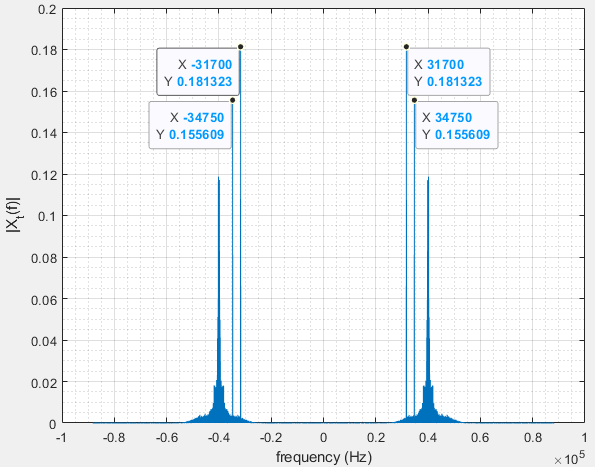
\includegraphics[width=0.6\linewidth]{./images/X_t.png}
\end{figure}
Si nota che, ignorando i due picchi a $\pm31700Hz$ e $\pm34750Hz$, la trasformata risulta essere composta da due pezzi identici, uno per valori negativi di frequenza e l'altro per valori positivi, entrambi simmetrici rispetto all'asse passante rispettivamente per $-40000Hz$ e $40000Hz$.\\
Questo è in accordo con la teoria, in quanto la trasformata di un segnale, con trasformata di Fourier $X(f)$, modulato con un coseno di frequenza $f_{0}$ è
\begin{equation}
	\frac{1}{2}[X(f - f_{0}) + X(f + f_{0})]
\end{equation}
Essendo $X_{t}(f)$ la trasformata di un segnale reale, si ha che il suo modulo è pari, dunque è simmetrico rispetto all'asse passante per $f=0$. Da ciò si deriva che $F_{m}=40000Hz$.\par
Ascoltando il segnale demodulato, si nota un disturbo dovuto a una componente ad alta frequenza. Essa deriva dai due picchi presenti nella trasformata $X_{t}(f)$, che nel segnale demodulato corrispondono a picchi alle frequenze $\pm5250Hz$ e $\pm8300Hz$. Per eliminare questo disturbo, si può filtrare il segnale originale con due notch filter, uno con $F_{filter} = 31700Hz$ e l'altro con $F_{filter} = 34750Hz$. In questo modo, i due picchi che danno origine al disturbo nel segnale demodulato scompaiono. Il segnale  $x(t)$ che si ottiene dalla demodulazione è più ovattato, in quanto il filtro elimina anche frequenze intorno alla $F_{filter}$ corrispondente.

Sia $x_{c}(t)$ il segnale ottenuto campionando $x(t)$ alla frequenza di $F_{c} = 29600Hz$. 

\end{document}
